\chapter{\ifenglish Background Knowledge and Theory\else ทฤษฎีที่เกี่ยวข้อง\fi}

\section{Ultra-Wideband (UWB)}
Ultra-Wideband (UWB) คือเทคโนโลยีไร้สายที่มีการใช้พลังงานต่ำซึ่งสามารถส่งข้อมูลจำนวนมากใน \\
ระยะทางสั้น ๆ ได้ โดยมีหลักการทำงาน ดังนี้\cite{sirin_uwb}
\begin{enumerate}
  \item \textbf{ขอบเขตความถี่และการควบคุมช่องสัญญาณ} \\
          UWB ทำงานภายในสเปกตรัมความถี่ที่อยู่ในช่วง 3.1 GHz ถึง 10.6 GHz โดยช่วงความถี่กว้างนี้ถูกออกแบบมาเพื่อรองรับ Orthogonal Frequency Division Multiplexing (OFDM) ซึ่งเป็นเทคนิคที่แบ่งสัญญาณออกเป็นหลายช่องสัญญาณย่อยที่มีความถี่ต่างกัน เพื่อลดการรบกวนระหว่างช่องสัญญาณและเพิ่มประสิทธิภาพในการรับส่งข้อมูล
  \item \textbf{การมอดูเลตพัลส์ การสื่อสาร และการส่งข้อมูล} \\
          UWB ใช้ พัลส์พลังงานสูงที่เกิดขึ้นในช่วงเวลาสั้นมาก แทนการใช้คลื่นต่อเนื่องเหมือนในเครือข่ายไร้สายทั่วไป โดยพัลส์เหล่านี้มีระยะเวลาวัดเป็นระดับ นาโนวินาที และถูกมอดูเลตเพื่อเข้ารหัสข้อมูล Time-Hopping Pulse Position Modulation (TH-PPM) เป็นเทคนิคที่ใช้ในการปรับตำแหน่งของพัลส์แต่ละชุดตามลำดับ เพื่อแทนค่าข้อมูลที่แตกต่างกัน ซึ่งช่วยให้การส่งข้อมูลมีความแม่นยำและลดการรบกวนระหว่างสัญญาณ
  \item \textbf{ประสิทธิภาพด้านพลังงานและความทนทานต่อสัญญาณรบกวน} \\
          การส่งข้อมูลแบบพัลส์ช่วยลด duty cycle ซึ่งช่วยให้ ประหยัดพลังงานและยืดอายุการใช้งานของแบตเตอรี่ ของอุปกรณ์ได้อย่างมีประสิทธิภาพ นอกจากนี้ การกระจายสัญญาณในช่วงความถี่กว้าง และมักจะอยู่ต่ำกว่าระดับสัญญาณรบกวนของระบบ RF ทั่วไป ทำให้ UWB มีความสามารถในการต้านทานการรบกวนจากสัญญาณสะท้อน (multipath interference) และการรบกวนจากช่องสัญญาณร่วม (co-channel disturbances) ได้ดี ซึ่งช่วยให้การสื่อสารมีเสถียรภาพและมีประสิทธิภาพในสภาพแวดล้อมที่มีอุปกรณ์ไร้สายหนาแน่น
  \item \textbf{ตัวชี้วัดตำแหน่งและเทคนิคการเข้าถึง} \\
          UWB สามารถวัดระยะทางได้อย่างแม่นยำ โดยอาศัยความเร็วของคลื่นแม่เหล็กไฟฟ้าและเวลาที่พัลส์เดินทางระหว่างตัวส่งและตัวรับ โดยใช้หลักการ Time of Arrival (ToA) และ Time Difference of Arrival (TDoA) ซึ่งช่วยให้สามารถระบุตำแหน่งได้ในระดับเซนติเมตร
\end{enumerate}
\subsection{Time of Flight (ToF) และ Time Difference of Arrival (TDoA)}
ในการประยุกต์ใช้ Ultra-Wideband สำหรับการวัดระยะทาง สามารถใช้หลักการ Time of Flight (ToF) 
ซึ่งเป็นการวัดเวลาที่สัญญาณใช้ในการเดินทางจากตัวส่งไปยังตัวรับ โดยอาศัยความเร็วของคลื่นแม่เหล็กไฟฟ้าเป็นค่าคงที่ \cite{gezici2005localization}

ในระบบที่ใช้งานจริง เช่น Two-Way Ranging (TWR) จะมีการส่งสัญญาณไป-กลับระหว่างอุปกรณ์สองตัว 
เพื่อลดผลกระทบจากความคลาดเคลื่อนของนาฬิกา (clock offset) ทำให้สามารถคำนวณระยะทางได้โดยไม่จำเป็นต้องมีการซิงโครไนซ์เวลาที่แม่นยำ \cite{decawave_appnote}

นอกจากนี้ ยังมีเทคนิค Time Difference of Arrival (TDoA) ซึ่งใช้ความแตกต่างของเวลาที่สัญญาณมาถึงอุปกรณ์หลายตัว 
ในการคำนวณตำแหน่งของวัตถุ โดยต้องอาศัยการซิงโครไนซ์เวลาระหว่างอุปกรณ์อย่างแม่นยำ

\subsection{สมการการคำนวณระยะทาง}
การคำนวณระยะทางจาก Time of Flight สามารถแสดงได้ด้วยสมการดังนี้
\begin{equation}
d = c \times t
\end{equation}
โดยที่ \( d \) คือ ระยะทาง (เมตร), \( c \) คือ ความเร็วของแสง (\(3 \times 10^8\) เมตรต่อวินาที), และ \( t \) คือเวลาเดินทางของสัญญาณ
สำหรับระบบ Two-Way Ranging (TWR) สามารถเขียนสมการได้เป็น

\begin{equation}
d = \frac{c \times t_{round}}{2}
\end{equation}
โดยที่ \( t_{round} \) คือเวลาไป-กลับของสัญญาณระหว่างอุปกรณ์ทั้งสอง

\subsection{ปัจจัยที่ส่งผลต่อความคลาดเคลื่อนในการวัดระยะทาง}
แม้ว่า UWB จะมีความแม่นยำสูง แต่ยังมีปัจจัยหลายประการที่ส่งผลต่อความคลาดเคลื่อนของการวัดระยะทาง ดังนี้
\begin{enumerate}
  \item \textbf{Non-Line-of-Sight (NLOS)} \\
  เกิดขึ้นเมื่อสัญญาณไม่สามารถเดินทางเป็นเส้นตรงระหว่างตัวส่งและตัวรับได้ 
  เช่น ในกรณีที่มีต้นไม้หรือสิ่งกีดขวาง ทำให้สัญญาณต้องสะท้อนหรือเลี้ยวเบน ส่งผลให้ระยะทางที่คำนวณได้มีค่ามากกว่าความเป็นจริง \cite{alavi2016uwb}

  \item \textbf{Multipath Propagation} \\
  สัญญาณอาจสะท้อนจากพื้นหรือวัตถุรอบข้าง ทำให้ตัวรับได้รับสัญญาณหลายเส้นทาง 
  ซึ่งอาจทำให้ระบบเลือกสัญญาณที่ไม่ใช่เส้นทางตรง ส่งผลต่อความแม่นยำ \cite{gezici2005localization}

  \item \textbf{Clock Drift และ Synchronization Error} \\
  ความคลาดเคลื่อนของนาฬิกาในอุปกรณ์ส่งและรับ อาจทำให้การวัดเวลา ToF ผิดพลาดได้ โดยเฉพาะในระบบ TDoA \cite{decawave_appnote}

  \item \textbf{สภาพแวดล้อมและสัญญาณรบกวน} \\
  สภาพแวดล้อมที่มีวัตถุจำนวนมาก เช่น ป่าไม้หนาแน่น อาจทำให้เกิดการสะท้อนของสัญญาณจำนวนมาก 
  ซึ่งส่งผลต่อความแม่นยำในการวัดระยะทาง
\end{enumerate}

\section{อากาศยานไร้คนขับ (Unmanned Aerial Vehicle :UAV)}
อากาศยานไร้คนขับ หรือ UAV (Unmanned Aerial Vehicle) ซึ่งมักเรียกกันว่า โดรน (Drone) เป็นอากาศยานที่สามารถบินได้โดยไม่ต้องมีนักบินควบคุมภายในเครื่อง สามารถทำงานได้ผ่านการควบคุมระยะไกลหรือระบบอัตโนมัติ โดย UAV ถูกพัฒนาให้มีหลากหลายขนาดและฟังก์ชันการใช้งานที่แตกต่างกัน \\

UAV ถูกนำมาใช้อย่างแพร่หลายในหลายภาคส่วน เช่น การทหาร, การสันทนาการ, และเชิงพาณิชย์ \cite{thaipbs_article} โดยสามารถใช้ในภารกิจต่าง ๆ เช่น การสอดแนม, การลาดตระเวน, การสำรวจพื้นที่, และการเฝ้าระวังสภาพแวดล้อม ปัจจุบันโดรนถูกติดตั้งด้วยอุปกรณ์ที่ทันสมัย เช่น กล้องความละเอียดสูง, กล้องอินฟราเรด, และเซ็นเซอร์ต่าง ๆ เพื่อช่วยเพิ่มประสิทธิภาพในการทำงาน \cite{gistda_news} \\

นอกจากนี้ UAV ยังสามารถประยุกต์ใช้ในสถานการณ์ฉุกเฉิน เช่น การสำรวจพื้นที่ประสบภัยพิบัติ, การตรวจสอบไฟป่า, และการเฝ้าระวังมลพิษทางทะเล ทำให้ UAV กลายเป็นเทคโนโลยีสำคัญที่ช่วยเพิ่มขีดความสามารถในการเก็บข้อมูลและตัดสินใจในสภาพแวดล้อมที่ซับซ้อน

\section{3D Printing}
เทคโนโลยีการพิมพ์ 3 มิติ (3D Printing) คือ เทคโนโลยีที่ใช้ในกระบวนการขึ้นรูปวัตถุ 3 มิติขึ้นจากโปรแกรมคอมพิวเตอร์ ด้วยการเติมเนื้อวัสดุเข้าไปทีละชั้น โดยคอมพิวเตอร์จะทำหน้าที่ควบคุมกระบวนการในทุกขั้นตอน\cite{depa_3d_printing} อาศัยหลักการ คือแปลงข้อมูลดิจิตอลที่เป็นแบบจำลอง 3 มิติ หั่นออกมาเป็น ข้อมูล 2 มิติ หลายๆชั้น ขั้นตอนนี้เรียกว่า การแบ่งชั้น (Slicing) จากนั้นส่งข้อมูลไปยังเครื่องพิมพ์ ให้เริ่มพิมพ์ชิ้นงานทีละชั้นจนได้แบบจำลองสามมิติตามที่ได้ออกแบบไว้ ซึ่งการพิมพ์ลักษณะนี้เราสามารถเรียกได้ว่าการผลิตแบบเติมเนื้อ (Additive manufacturing, AM)\cite{sync_innovation_3dprinting} ซึ่งมีข้อดีกว่าเทคนิคการขึ้นรูปทั่วไปคือ การสูญเสียวัตถุดิบที่น้อยกว่า \\
เทคโนโลยี 3D Printing จำแนกตามกระบวนการที่แตกต่างกันได้เป็น 3 ประเภทหลัก ได้แก่\cite{depa_3d_printing}
\begin{itemize}
  \item \textbf{Fused Deposition Modeling (FDM)} เป็นการนำวัสดุที่จะใช้ขึ้นรูปมาหลอมละลายเป็นเส้น 
   (Filament) แล้วฉีดออกมาเป็นชิ้นงานขึ้นรูปทีละชั้น ข้อดีของเทคนิคนี้คือ ราคาถูก หาซื้อได้ง่าย 
   ใช้งานง่ายและใช้ได้กับวัสดุที่หลากหลาย แต่ความละเอียดในการพิมพ์และระยะเวลาที่ใช้ยังมี 
   ประสิทธิภาพต่ำกว่าการพิมพ์แบบอื่น
   \item \textbf{Stereolithography (SLA)} เป็นเทคโนโลยีการพิมพ์ 3 มิติชนิดแรกที่เกิดขึ้น เป็นเทคนิคที่ใช้แสง 
   อัลตราไวโอเลต ยิงใส่ผิวเรซินของวัสดุให้เกิดการแข็งตัวทีละชั้น ข้อดีของเทคนิคนี้คือ ทำให้ได้ชิ้นงานที่มีควาละเอียดสูง ผิวเรียบ ความเร็วในการพิมพ์ไม่ลดลงเมื่อพิมพ์งานทีละหลายชิ้น แต่ข้อเสียคือ เรซินเหลวที่ใช้ในการพิมพ์ค่อนข้างเลอะเทอะ เหม็น และเป็นอันตรายถ้าสูดดมเข้าไปในปริมาณมาก
   \item \textbf{Selective Laser Sintering (SLS)} เป็นการใช้แสงเลเซอร์ยิงลงบนพื้นผิววัสดุให้วัสดุเกิดการหลอมเหลวเป็นเนื้อเดียวกัน โดยจะเลือกยิงเฉพาะจุด ข้อดีของเทคนิคนี้คือ ชิ้นงานที่ได้มีความแข็งแรงคงทนแต่ราคาของเครื่องพิมพ์ยังค่อนข้างสูง และวัสดุที่ใช้กับเครื่องพิมพ์แบบนี้ได้มีค่อนข้างจำกัดเมื่อเทียบกับเครื่องพิมพ์แบบอื่นๆ
\end{itemize}
ในส่วนของรายละเอียดขั้นตอน การสร้างชิ้นงานจากเครื่องพิมพ์สามมิติมี ดังนี้ \cite{trueplookpanya_education}
\begin{enumerate}
  \item \textbf{การสร้างแบบจำลองสามมิติ (3D Modelling)} \\
  เป็นขั้นตอนเริ่มต้นของการใช้งานโดยการ ใช้โปรแกรมทางคอมพิวเตอร์หรือ CAD เขียนแบบชิ้นงานออกมาเป็นภาพร่าง สามมิติตามขนาดและรูปร่างที่ต้องการ ซึ่งปัจจุบันสามารถหาโปรแกรมฟรีแวร์
  และราคาถูกได้ง่ายมาก เช่น Autodesk Fusion , Blender, TinkerCAD หรือ แม้กระทั่ง 3D Paint หลังจากนั้นให้ทำการบันทึกไฟล์ (SAVE) หรือ export ออกมาเป็นไฟล์สามมิติ เพื่อให้มองเห็นภาพร่างชิ้นงานที่ต้องการในรูปแบบของ ไฟล์ภาพสามมิติ ก่อนทำการสั่งพิมพ์ด้วยเครื่องพิมพ์
  \item  \textbf{การพิมพ์สามมิติ (Printing)} \\
  เมื่อได้ไฟล์ภาพสามมิติเรียบร้อยแล้วในขั้นตอนนี้จะเป็นการสั่งพิมพ์ผ่านซอฟต์แวร์จัดการไฟล์ดิจิทัล 
  โดยเครื่องพิมพ์สามมิติจะทำการหลอมวัสดุ พิมพ์และทำการพิมพ์ตามงานที่ต้องการ โดยพิมพ์ออกมาเป็นแนวระนาบและเพิ่มรายละเอียดเป็นชั้นซ้อนทับกันไปเรื่อยๆตามสเกลของชิ้นงานที่ต้องการ 
  \item \textbf{การตกแต่งชิ้นงานหลังการพิมพ์ (Post Processing)} \\
  สำหรับในส่วนของขั้นตอนนี้จะเป็นการ ตกแต่งชิ้นงานหลังการพิมพ์ ซึ่งผู้ใช้สามารถดำเนินการขัด 
  (polishing) ทำสี (painting) หรือนำชิ้นงานหลาย ๆ ชิ้นมาประกอบหรือติดกาวเข้าด้วยกัน  โดยแต่ละเทคโนโลยีของเครื่องพิมพ์สามมิติมักจะมีขั้นตอนที่อาจมีความแตกต่างกันไป
\end{enumerate}

ปัจจุบัน เทคโนโลยี 3D Printing ได้ถูกนำไปใช้ในงานหลากหลายประเภท เช่น การแพทย์อุตสาหกรรม สถาปัตยกรรม รวมถึงวัสดุในการขึ้นรูปก็มีความหลากหลายมากขึ้นตามวัตถุประสงค์ของงานด้วย นอกจากนี้ ความนิยมในการใช้ 3D Printer มีแนวโน้มที่จะขยายตัวอย่างต่อเนื่อง เนื่องจากต้นทุนการผลิตที่ลดลง เงินลงทุนสนับสนุนการวิจัยและพัฒนาจากภาครัฐ การขยายตัวของตลาดที่มีผู้ผลิตรายใหม่เพิ่มขึ้น\cite{depa_3d_printing} ทั้งนี้ 3D Printing เป็นเทคโนโลยีที่เหมาะสำหรับการสร้าง ตัวยึด (Bracket) หรือ ตัวล็อกโมดูล (Mount) บนโดรน เนื่องจากมีความยืดหยุ่นในการออกแบบและน้ำหนักเบา ซึ่งช่วยลดผลกระทบต่อเสถียรภาพการบินของโดรน
\\
\begin{figure}[htbp]
        \centering
        \begin{minipage}{0.45\textwidth}
                % 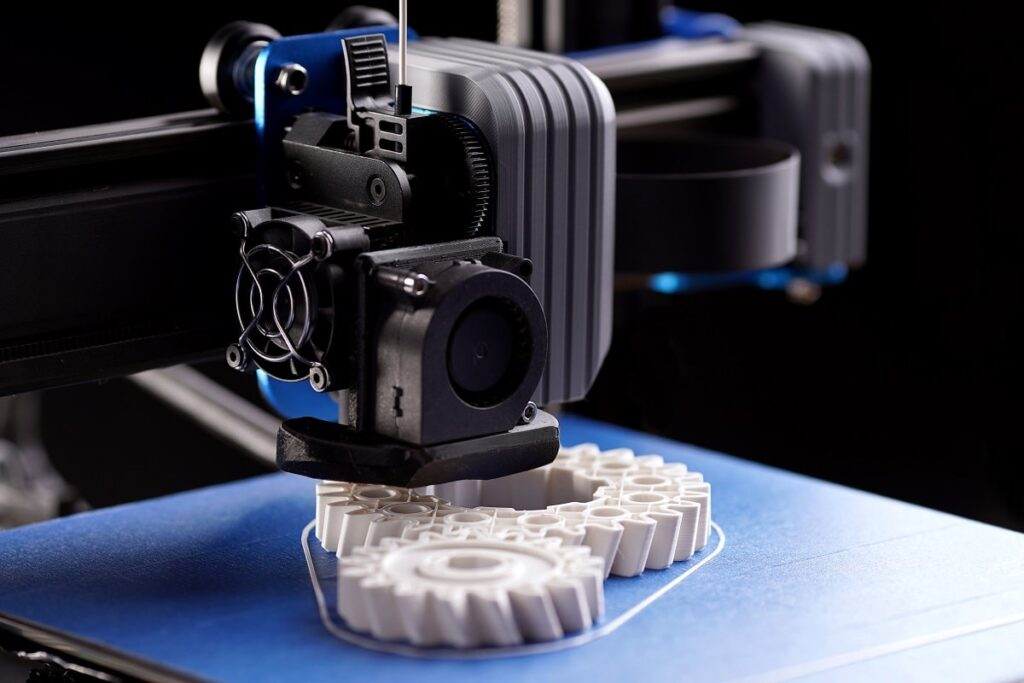
\includegraphics[width=\linewidth]{fig/3D.jpg} 
                \caption{ตัวอย่างการพิมพ์ 3D}
        \end{minipage}
        \hfill
        \begin{minipage}{0.45\textwidth}
                % 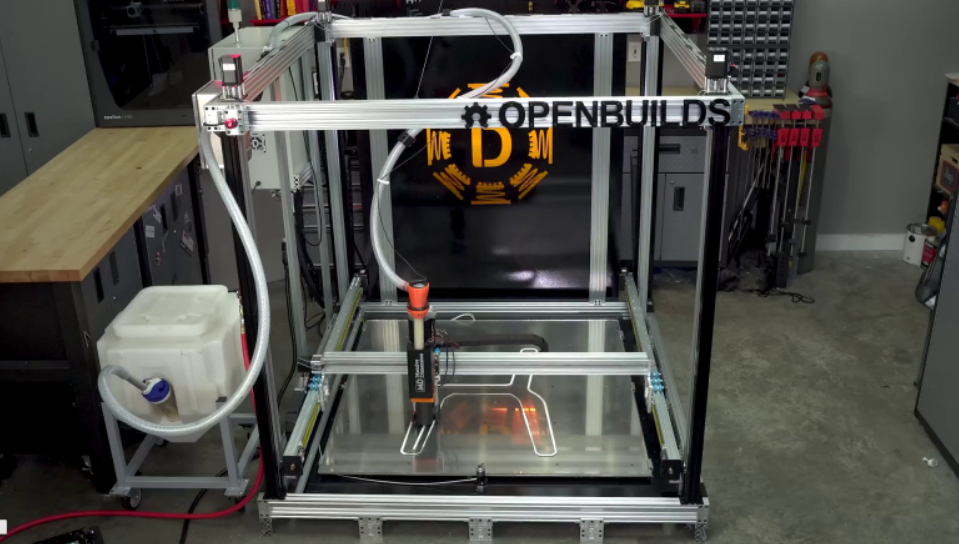
\includegraphics[width=\linewidth]{fig/3D2.png} 
                \caption{เครื่องพิมพ์ 3D}
        \end{minipage}
\end{figure}